\chapter{Entwurf}
\label{ch:3}

\section{Grobentwurf: Subsysteme}
\label{sec:3.1}
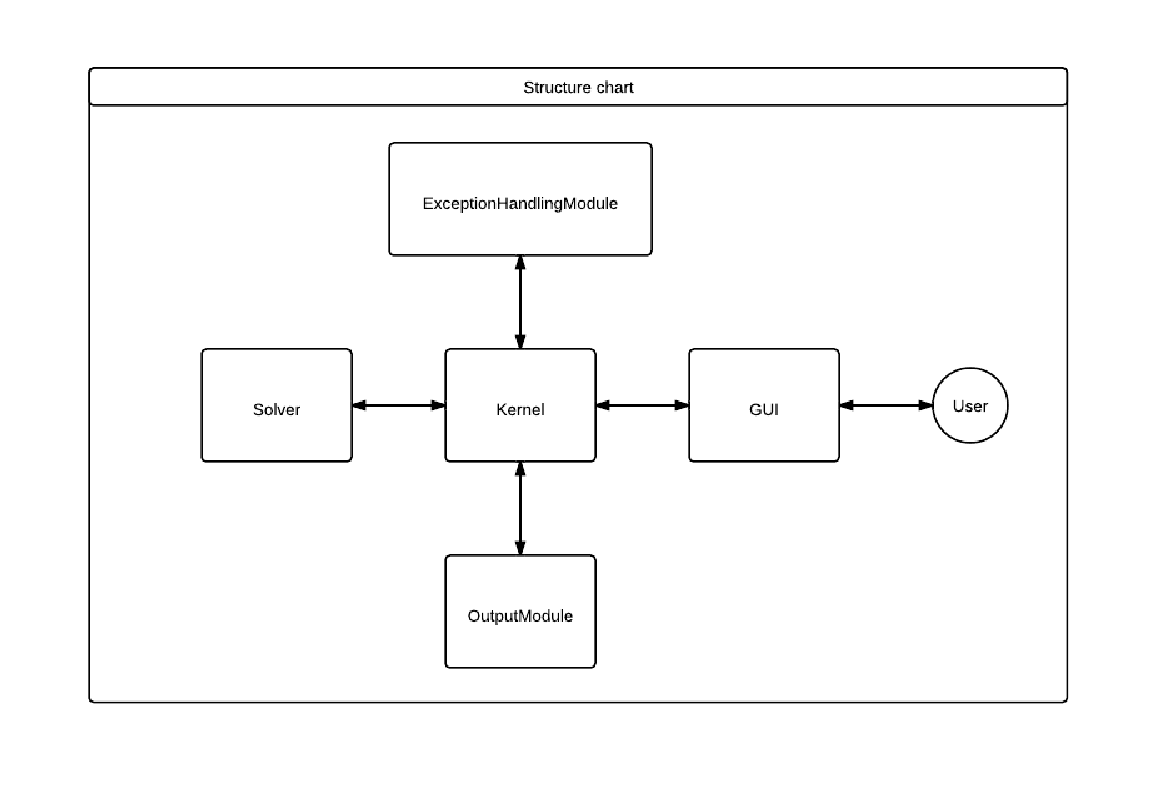
\includegraphics[width=6in,keepaspectratio=true]{figures/StructureDiagGyroSim.eps}

%% \subsection{Statik}

%% \subsection{Dynamik}

\section{Detailentwurf: Klassen}
\label{sec:3.2}
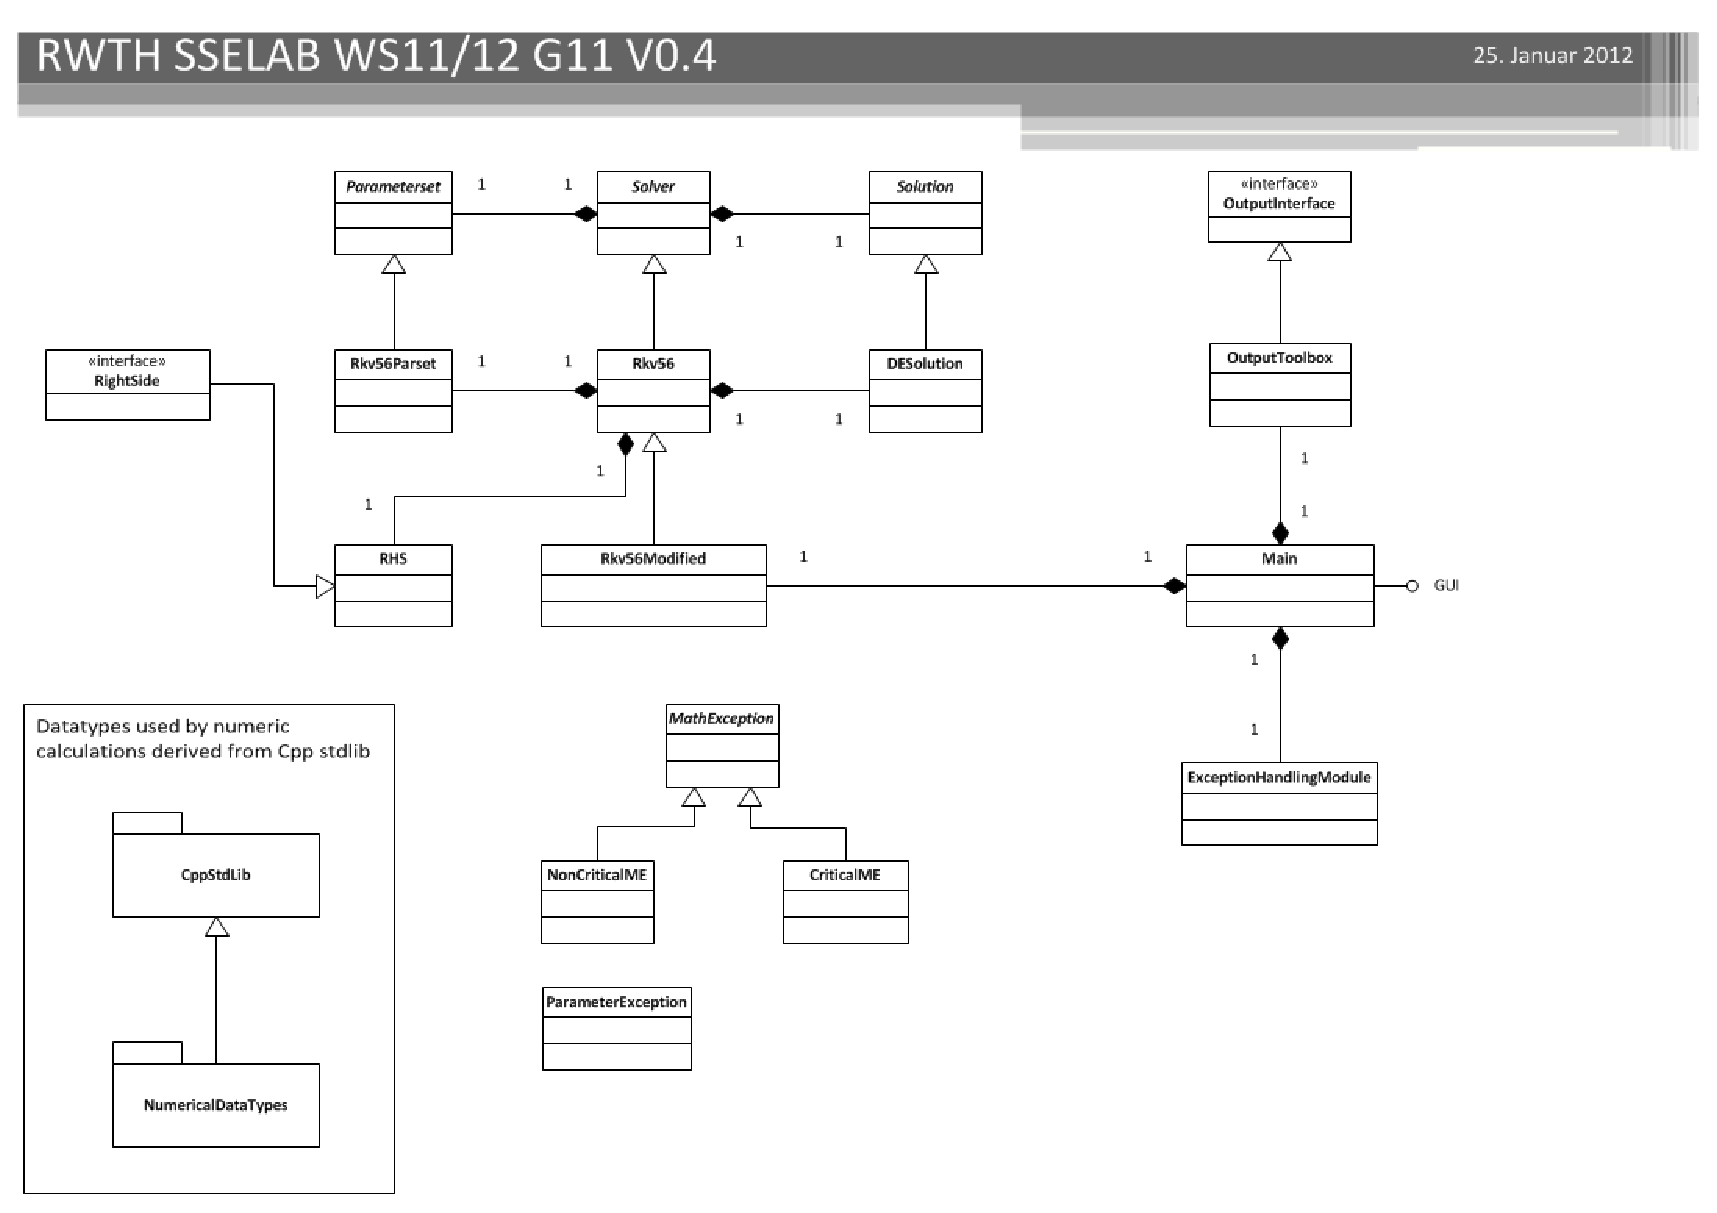
\includegraphics[width=6in,keepaspectratio=true]{figures/RWTH_SSELAB_WS1112_CLASSES.eps}

\subsection*{StepperDopr853 ? Dormand-Prince 853 method}
Der Dopr853 Algorithmus ist ein Algorithmus aus der Familie der Runge-Kutta Algorithmen der Ordnung 8.  F�r jeden Schritt werden 12 Auswertungen der rechten Seite des DGL ben\o"tigt.
Der urspr\"ungliche Algorithmus nutzte eine Fehlersch\"atzung der Ordnung 6, was sich allerdings in einigen F\"allen als unzureichend herausstellte, da dieser Fehlersch\"atzer jeweils die letzte Auswertung nicht ber\"ucksichtigte. Hairer, N\"orsett und Wanner1 konstruierten Absch\"atzungen der f\"unften und dritten Ordnung, die auch den letzen Punkt ber\"ucksichtigen. Der Fehler kann also \"uber \\
$err = err_5 \frac{err_5}{sqrt{(err_3)^2+0.01(err_5)^2}}$ \\
abgesch\"atzt werden. 

Die meiste Zeit �ber gilt $err_5 << err_3$ und damit $err=O(h^8)$. \medskiip

StepperDopr853 wurde als Mehrschrittverfahren mit fehlergesteuerter Schrittweitensteuerung implementiert, die neben dem gesch\"atzten Fehler auch noch die Erhaltungsgr\"o\sse \\
$IR\dot\phi\sin^2\theta+I_3(R\cos\theta-a)(\dot\phi\cos\theta+\dot\psi) = const =: G$ \\
ber\"ucksichtigt. ($\Delta G$ pro Schritt $< 1E-6$ ).
Der L\"oser unterst\u"tzt sowohl eine dichte Ausgabe \textit{dense output}, als auch die Ausgabe von n \"aquidistant verteilten Werten. 

\textit{Frei nach NumericalRecipes3rdEdition ? Chapter 17.2.4 Dopr853 ? An Eight-Order Method

Implementierung nach 
Numerical Recipes Software 2007, ?Routine Implementing an Eighth-order Runge-Kutta Method,? 
Numerical Recipes Webnote No. 20, at http://www.nr.com/webnotes?20\footnote{Hairer, E., N�rsett, S.P., and Wanner, G. 1993, Solving Ordinary Differential Equations I. Nonstiff 
Problems, 2nd ed. (New York: Springer). Fortran codes at 
http://www.unige.ch/~hairer/software.html }}








\subsection{Statik}
\subsection{Dynamik}
\section{Graphical User Interface}
\label{sec:3.3}
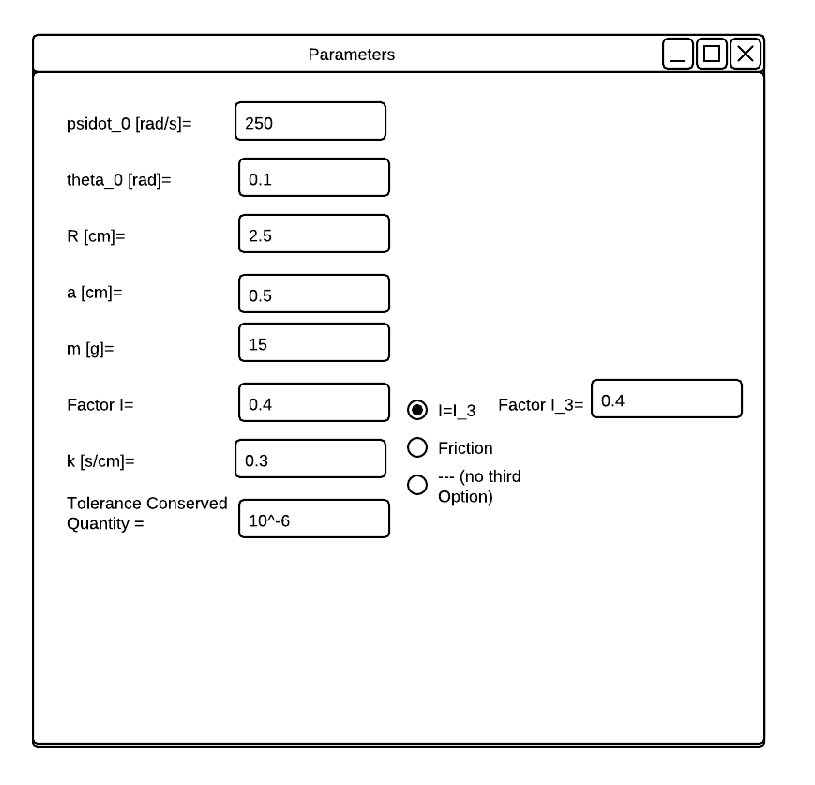
\includegraphics[width=6in,keepaspectratio=true]{figures/GUIParameterInputForm.eps}
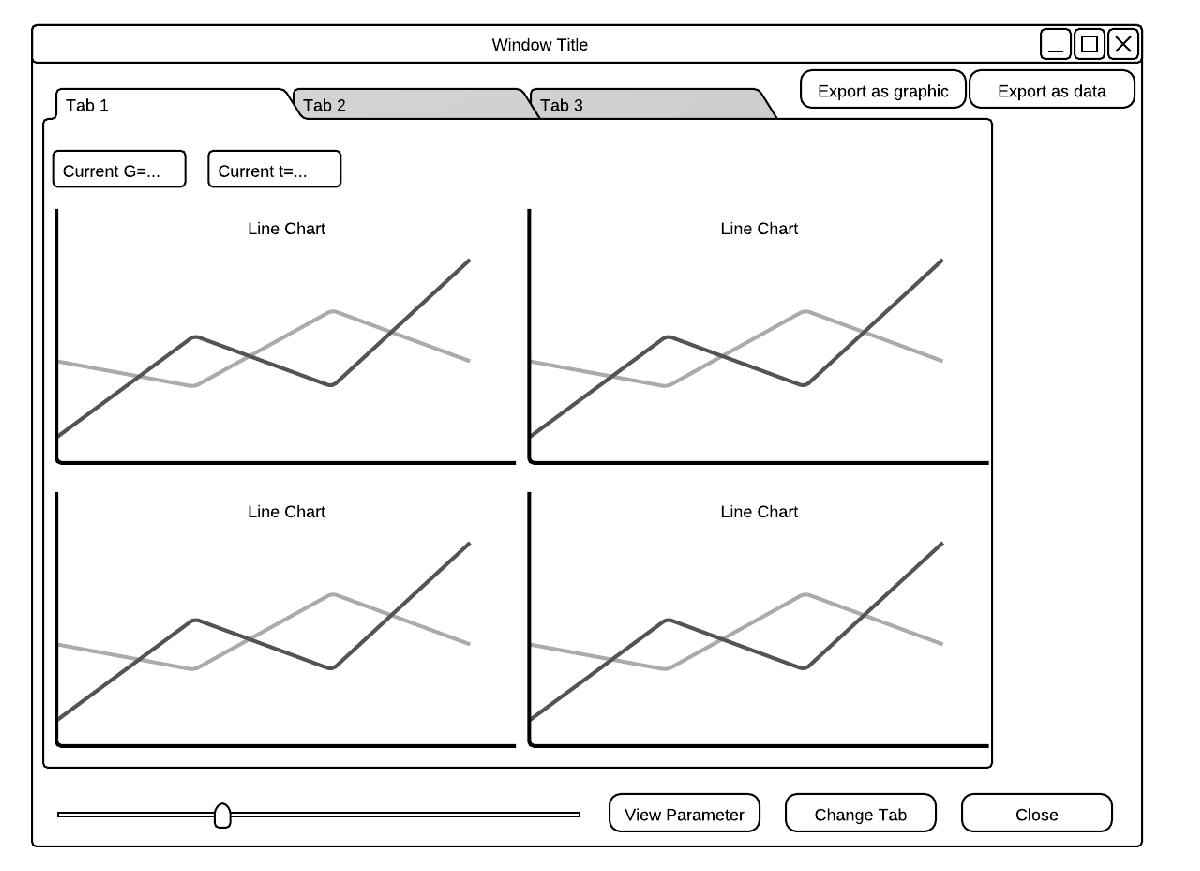
\includegraphics[width=6in,keepaspectratio=true]{figures/GUIDisplayForm.eps}
\section{Use-Case-Diagramm}
\label{sec:3.4}
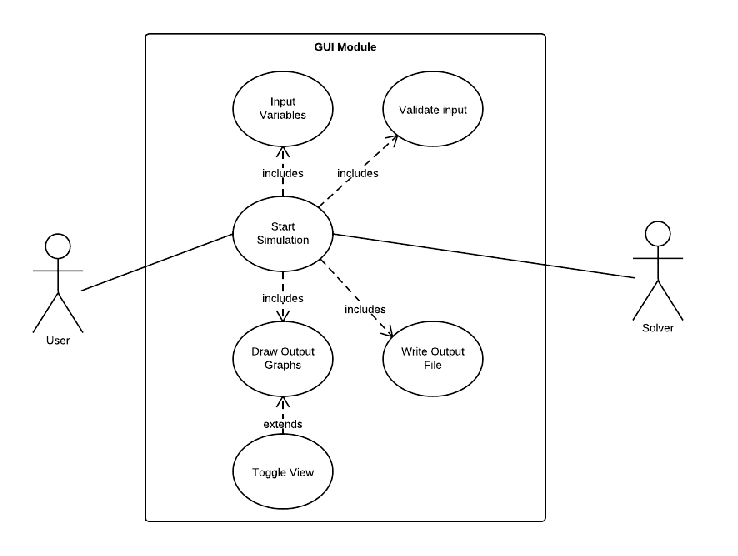
\includegraphics[width=6in,keepaspectratio=true]{figures/UseCaseTippeTop.eps}

